\chapter{Computer vision}
\section{Requirements of objective}
Automated asparagus harvesting necessitates reliable perception to locate, assess, and safely manipulate spears within complex field conditions. Computer vision provides the sensing and interpretation capabilities required to: (i) detect spears amidst cluttered foliage and soil background; (ii) estimate ripeness or cut-readiness based on geometric and visual cues; (iii) localize targets in three dimensions for tool approach and cutting; and (iv) operate robustly under variability in illumination, occlusions, plant morphology, and weather. In this context, perception performance directly constrains the achievable throughput, product quality, and operational safety of the harvesting system.

The primary requirements are summarized as follows:
\begin{itemize}
  \item \textbf{Detection accuracy}: High precision and recall to minimize missed harvestable spears and false positives that could cause damage.
  \item \textbf{Spatial localization}: Centimeter-level 3D pose (position and, where relevant, orientation) sufficient for motion planning of the end effector.
  \item \textbf{Readiness assessment}: Discrimination between harvestable and non-harvestable spears using measurable features (e.g., height above soil, thickness, tip morphology).
  \item \textbf{Environmental robustness}: Tolerance to shadows, direct sunlight, moisture, dust, and partial occlusions from leaves or neighboring spears.
  \item \textbf{Computational efficiency}: Near real-time inference compatible with the platform's compute and energy budgets.
  \item \textbf{Scalability and maintainability}: Methods that generalize across cultivars, growth stages, and fields with limited re-calibration.
  \item \textbf{Safety and compliance}: Conservative behavior near humans and plants; perception outputs support fail-safe planning and execution.
\end{itemize}

To meet these requirements, this work uses camera-based sensing for both 2D appearance cues and 3D geometric reasoning. The approach integrates image acquisition, camera calibration, point-cloud generation, and segmentation to produce actionable targets for manipulation.

\section{Dataset collection and  model training}
A web-sourced image corpus of 200 asparagus scenes was curated and annotated using the COCO methodology to enable instance-level learning. 
Images were intentionally selected to span challenging, field-relevant variability, including cluttered arrangements and occlusions among 
spears, out-of-focus and mild motion-blur cases, diverse viewpoints and backgrounds, and a broad range of illumination conditions (e.g., 
backlighting, hard shadows, and mixed artificial/ambient lighting). The dataset was partitioned at the image level into non-overlapping 
training (80\%) and test (20\%) splits while preserving the distribution of scene characteristics across splits to reduce evaluation bias.
This diversity is intended to promote robustness and generalization of the Detectron2 models trained in subsequent experiments (see Figure~\ref{fig:dataset_samples}).

Training uses Detectron2's Mask R-CNN with a ResNet-50 backbone and Feature Pyramid Network ,
initialized from COCO-pretrained weights. No validation dataset is attached to the training loop. The model is optimized on CPU with two
 data-loading workers, a base learning rate of \(2.5\times10^{-4}\), and a fixed schedule without decay for a total of 300 iterations. The ROI heads
 are configured for a single foreground category (asparagus spear), with batch size of 128 to balance computation and convergence
 stability for this dataset size. The total training time on Google Colab was approximately 5.3 hours.

\begin{figure}[H]
\centering
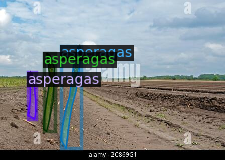
\includegraphics[width=0.48\linewidth]{asp_sample_1.png}\hfill
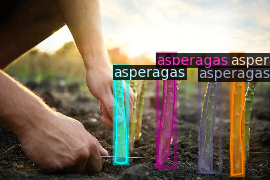
\includegraphics[width=0.48\linewidth]{asp_sample_2.png}\\[0.5em]
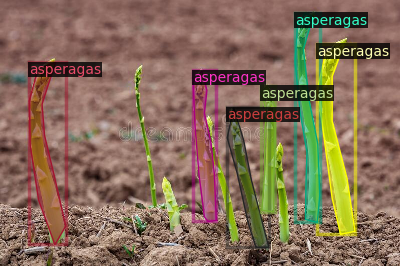
\includegraphics[width=0.48\linewidth]{asp_sample_3.png}\hfill
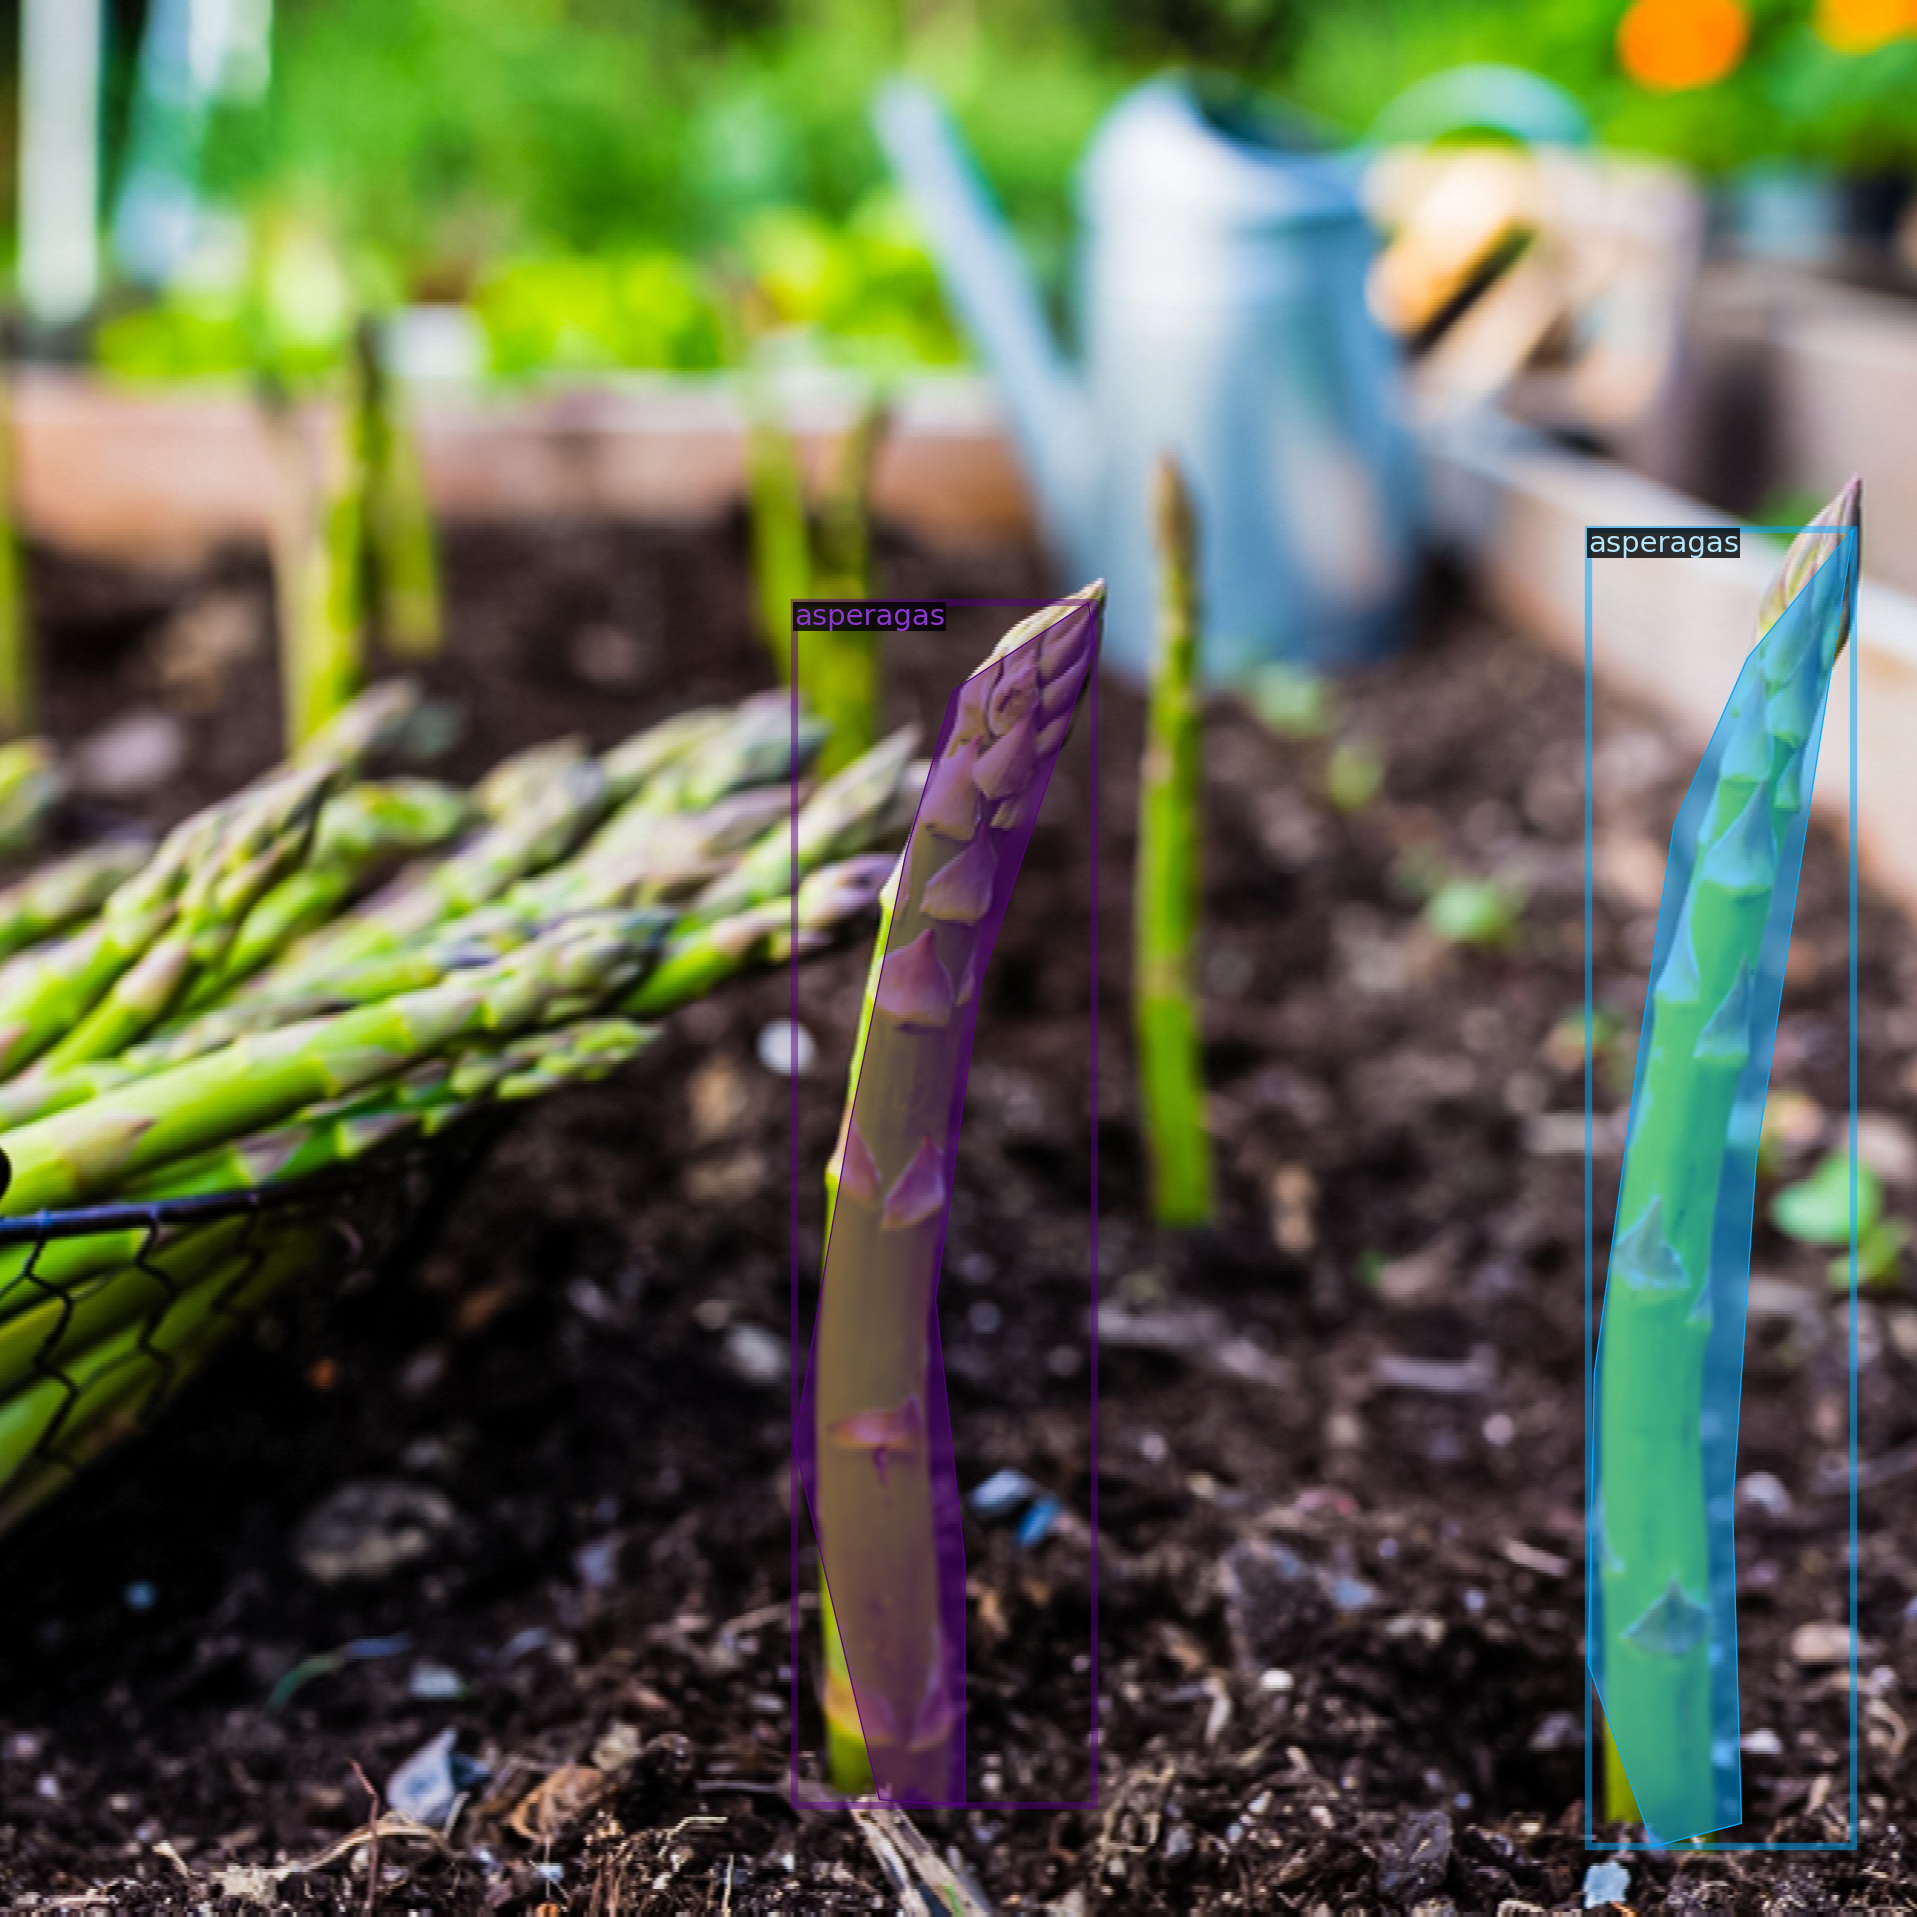
\includegraphics[width=0.48\linewidth]{asp_sample_4.png}
\caption{Representative training samples illustrating variability in clutter, focus, viewpoint, background, and illumination within the dataset described above.}
\label{fig:dataset_samples}
\end{figure}


After training, the model is exported as a TorchScript artifact for deployment and used for inference on the held-out test split. A confidence
threshold of 0.85 is applied for instance selection. On the test dataset, the model achieves an overall detection accuracy above 98.4\%.
Representative qualitative results are shown in Figure~\ref{fig:inference_results}.

\begin{figure}[H]
\centering
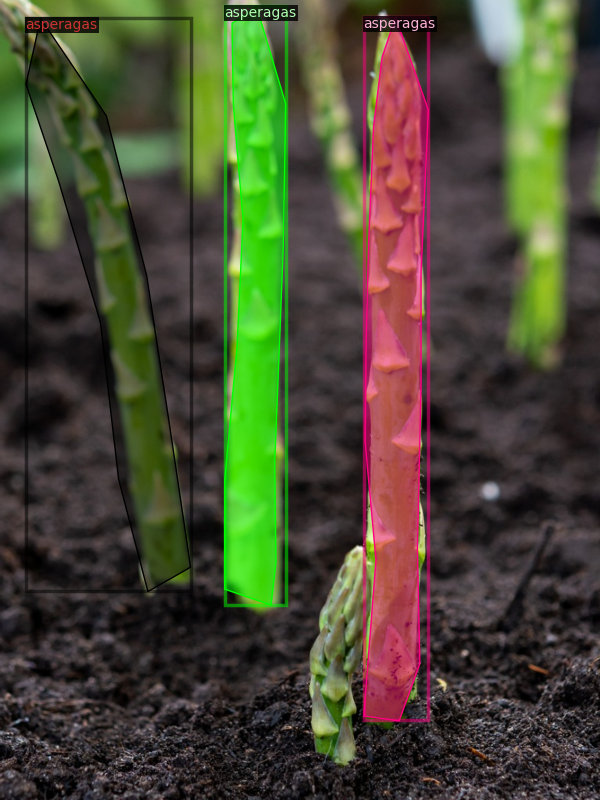
\includegraphics[width=0.48\linewidth]{test_image.png}\hfill
\includegraphics[width=0.48\linewidth]{\detokenize{test_image (2).png}}
\caption{Qualitative inference results on held-out test images. Detected asparagus spears are shown with instance masks and bounding boxes, illustrating robust performance under varied backgrounds and illumination.}
\label{fig:inference_results}
\end{figure}



\section{camera setup in lab environment}
 The laboratory configuration replicates typical field viewing geometry while providing controlled and repeatable imaging conditions. The camera is 
 rigidly mounted on an aluminum extrusion frame using a vibration-damped bracket, with the optical axis oriented obliquely toward the 
 crop bed at an incidence angle of approximately 25--35 degrees. The working distance is set such that a single frame covers the full 
 spear length from soil interface to tip with a 10--20\% margin, ensuring both context and sufficient pixel density for fine structures.

 Intrinsic calibration (focal length, principal point, and lens distortion) is performed following a standard  procedure advised by 
 the manufacturer of the camera; extrinsic calibration to the robot base is obtained via hand--eye calibration with a fixed calibration
  artifact placed at known locations within the workspace.  All transforms are stored and validated at the beginning of each session.

 Illumination is standardized using diffuse LED panels positioned to minimize specular highlights and cast shadows.

 Image acquisition is configured at a constant resolution and frame rate suitable for downstream processing latency. A measurment tape is
 used  in the field of view for periodic verification of metric accuracy. All data are logged with session metadata (calibration parameters, lighting
 settings, and environmental notes) to enable reproducibility. A figure illustrating the physical arrangement of the camera, lighting,
 and sample placement will be provided in this section.

\section{cloud point generation and processing}
Depth information is converted into a 3D point cloud through back-projection using the calibrated intrinsics. Each pixel with valid depth \(d\) at image coordinates \((u, v)\) is mapped to a camera-frame point \(\mathbf{p}_c = d\,K^{-1}[u\ v\ 1]^\top\), where \(K\) is the intrinsic matrix. Points are then transformed into the robot frame via the known extrinsics. Color values are optionally associated to each 3D point for appearance--geometry fusion.

To enhance downstream segmentation and localization, the raw cloud undergoes a processing pipeline:
\begin{itemize}
  \item \textbf{Region-of-interest filtering}: Crop to the expected bed and height range to reduce irrelevant background.
  \item \textbf{Downsampling}: Apply voxel-grid filtering to obtain approximately uniform density and lower computation.
  \item \textbf{Ground removal}: Fit and subtract the soil plane using robust estimators (e.g., RANSAC) to isolate above-ground structures.
  \item \textbf{Outlier suppression}: Remove statistical outliers based on neighborhood distances to improve surface smoothness.
  \item \textbf{Normal estimation}: Compute local surface normals for geometric descriptors and later shape reasoning.
\end{itemize}
The resulting cloud provides a compact, denoised representation suitable for spear segmentation and 3D pose extraction.

\section{segmentation}
Segmentation partitions the sensed scene into spear and non-spear regions and, when required, separates individual spears (instance-level segmentation). Two complementary strategies are considered depending on sensing modality and compute budget:
\begin{enumerate}
  \item \textbf{Geometry-first 3D segmentation}: Cluster the filtered point cloud using Euclidean or density-based methods, followed by geometric constraints on cluster height, thickness, and verticality to retain spear-like structures. This approach is robust to color variation and leverages ground-removed geometry.
  \item \textbf{Learning-based image segmentation}: Apply a convolutional neural network for semantic or instance segmentation in 2D (e.g., encoder--decoder architectures). The 2D masks are lifted to 3D via the registered depth to obtain per-spear point sets. This approach captures fine visual cues and handles partial occlusions when sufficient training data are available.
\end{enumerate}

Post-processing includes morphological smoothing, non-maximum suppression for overlapping hypotheses, and temporal association across frames when operating in motion. For each segmented spear, a 3D reference point (e.g., base point above soil or a cut point at a specified height) is estimated by fitting a simple parametric model to the cluster and intersecting with the soil plane. The final output is a set of target poses with confidence scores, which the planning module consumes for execution.

